\documentclass[12pt, twoside]{article}
\usepackage[letterpaper, margin=1in, head=30pt, headsep=0.1in]{geometry}
\usepackage[english]{babel}
\usepackage[utf8]{inputenc}
\usepackage{amsmath}
\usepackage{amsfonts}
\usepackage{amssymb}
\usepackage{tikz}
%\usetikzlibrary{quotes, angles}

\usepackage{graphicx}
\usepackage{enumitem}
\usepackage{multicol}

\newif\ifmeta
\metatrue %print standards and topics tags

\title{Regents Geometry}
\author{Chris Huson}
\date{October 2021}

\usepackage{fancyhdr}
\pagestyle{fancy}
\fancyhf{}
\renewcommand{\headrulewidth}{0pt} % disable the underline of the header
\raggedbottom


\fancyhead[LE]{\thepage}
\fancyhead[RO]{\thepage \\ Name: \hspace{4cm} \,\\}
\fancyhead[LO]{BECA / Dr. Huson / Geometry 04 Analytic Geometry}

\begin{document}

\subsubsection*{4.1 Midpoint Formula}
\begin{enumerate}
\item Given $\overleftrightarrow{AB}$ as shown on the number line, with $A=-3$ and $B=5$. 
\begin{enumerate}
  \item Find the length $AB$, writing an equation
  \item What is half the length? 
  \item Mark and label the midpoint $M$ between $A$ and $B$\\[1cm]
  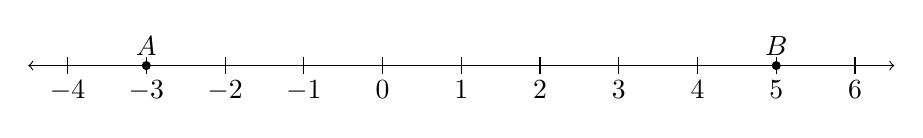
\begin{tikzpicture}
    \draw [<->] (-4.5,0)--(6.5,0);
    \foreach \x in {-4,...,6} %2 leading for diff!=1
      \draw[shift={(\x,0)},color=black] (0pt,-3pt) -- (0pt,3pt) node[below=5pt]  {$\x$};
      \draw [fill] (-3,0) circle [radius=0.05] node[above] {$A$};
      \draw [fill] (5,0) circle [radius=0.05] node[above] {$B$};
  \end{tikzpicture}
  \item Dr. Huson's commute is from 80th Street to 164th Street. On what block is he half way?
\end{enumerate}
  \vspace{3cm}
  
  \subsubsection*{The midpoint formula}
  Given $A(x_A,y_A)$, $B(x_B,y_B)$, midpoint $\displaystyle M = \left(\frac{x_A+x_B}{2}, \frac{y_A+y_B}{2}\right)$
\item On the graph below, draw $\overline{AB}$, with $A(2,3)$ and $B(8,5)$, labeling the end points. Determine and state the coordinates of the midpoint $M$ of $\overline{AB}$ and mark and label it on the graph.
\begin{flushright}
  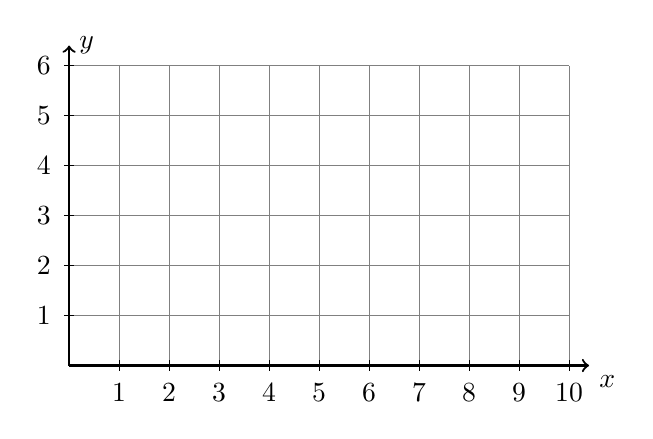
\begin{tikzpicture}[scale=.635]
    \draw [help lines] (0,0) grid (10,6);
    \draw [thick, ->] (0,0) -- (10.4,0) node [below right] {$x$};
    \draw [thick, ->] (0,0)--(0,6.4) node [right] {$y$};
    \foreach \x in {1,...,10}
    \draw[shift={(\x,0)}] (0pt,-3pt)--(0pt,3pt) node[below=5pt] {$\x$};
    \foreach \y in {1,...,6}
    \draw[shift={(0,\y)}] (-3pt,0pt)--(3pt,0pt) node[left=5pt] {$\y$};
  \end{tikzpicture}
\end{flushright}

\newpage
\item On the graph below, draw $\overline{AB}$, with $A(1,2)$ and $B(7,4)$, labeling the end points. Determine and state the coordinates of the midpoint $M$ of $\overline{AB}$ and mark and label it on the graph.
\begin{flushright}
  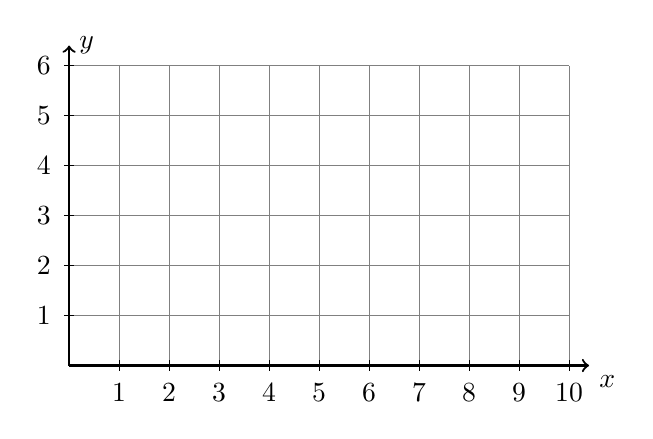
\begin{tikzpicture}[scale=.635]
    \draw [help lines] (0,0) grid (10,6);
    \draw [thick, ->] (0,0) -- (10.4,0) node [below right] {$x$};
    \draw [thick, ->] (0,0)--(0,6.4) node [right] {$y$};
    \foreach \x in {1,...,10}
    \draw[shift={(\x,0)}] (0pt,-3pt)--(0pt,3pt) node[below=5pt] {$\x$};
    \foreach \y in {1,...,6}
    \draw[shift={(0,\y)}] (-3pt,0pt)--(3pt,0pt) node[left=5pt] {$\y$};
  \end{tikzpicture}
\end{flushright}
\vspace{1cm}

\item Spicy Do Now: In  $\triangle ABC$ shown below, side $\overline{AC}$ is extended to point $D$ with \\ $m\angle DAB=(11x+12)^\circ$, $m\angle C=(3x+3)^\circ$, and $m\angle B=(9x+2)^\circ$. \\[0.25cm]
Find $m\angle BAC$.
\begin{flushright}
    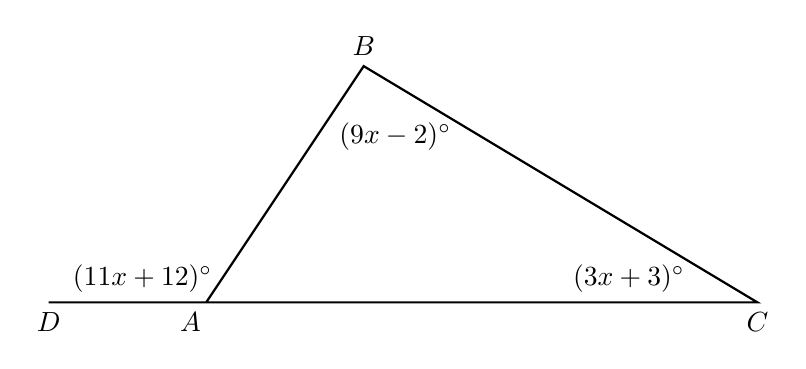
\begin{tikzpicture}
      \draw [thick](0,0)node[below]{$D$}--
        (1.8,0)node[below]{$A$}--
        (9,0)node[below]{$C$}--
        (4,3)node[above]{$B$} --(2,0);
        \node at (2.2,0)[above left]{$(11x+12)^\circ$};
        \node at (8.2,0)[above left]{$(3x+3)^\circ$};
        \node at (4.4,2.4)[below]{$(9x-2)^\circ$};
    \end{tikzpicture}
  \end{flushright} \vspace{1cm}

\item Given isosceles $\triangle RSU$ with $\overline{US} \cong \overline{RS}$. If $m\angle UST=150$ find $m\angle U$.
  \begin{flushright}
  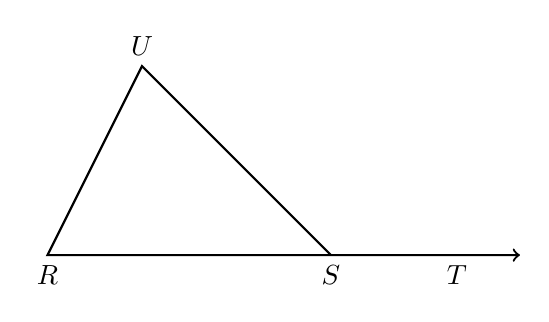
\begin{tikzpicture}[scale=0.8]
    %\draw [->, thick] (0,0)--(5,5);
    \draw [<-, thick] (8,0)--
      (7,0) node[below]{$T$}--
      (0.5,0) node[below]{$R$}--
      (2,3) node[above]{$U$}--
      (5,0) node[below]{$S$};
  \end{tikzpicture}
  \end{flushright}

\end{enumerate}
\end{document}

\item In  $\triangle ABC$ shown below, $m\angle A=(10x)^\circ$, $m\angle B=(16x-5)^\circ$, and $m\angle C=(2x+3)^\circ$. \\[0.25cm] 
  Find $m\angle A$. (show the check for full credit)
  \begin{flushright}
      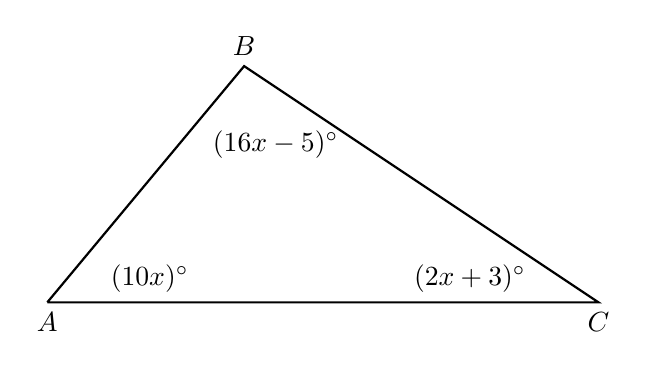
\begin{tikzpicture}
        \draw [thick]
          (2,0)node[below]{$A$}--
          (9,0)node[below]{$C$}--
          (4.5,3)node[above]{$B$} --(2,0);
          \node at (3.3,0)[above]{$(10x)^\circ$};
          \node at (8.2,0)[above left]{$(2x+3)^\circ$};
          \node at (4.9,2.3)[below]{$(16x-5)^\circ$};
      \end{tikzpicture}
    \end{flushright}